% ============================================================================
\section{Controlled Repair}
\label{sec:repair}

\subsection{One-factor ablation}
The earlier comparison changed scope, prior, scaling and the backoff fallback at
once. We replaced it with a one-factor-at-a-time ablation on dev, using the same
history-only candidate pools, allowed feedback rows and selection metric for every
cell. Table~\ref{tab:ablation} reports the retrieval-level top-1 proxy; the
generated panels confirm the selected finalist, not every cell.

\Table[!btp](width=\textwidth){Controlled one-factor-at-a-time ablation on dev
(retrieval-level top-1 proxy, 319 duplicate-panel and 312 prefix-panel queries).
Every cell uses the same history-only candidate pools, allowed feedback rows and
selection metric. ``Ratio'' is $\mathrm{SD}(\text{lift})/\mathrm{SD}(\text{retrieval
score})$ within the pool. Tuned Laplace uses $m=0.60$, cap $=0.15$ on the duplicate
panel and $m=1.00$, cap $=0.05$ on the prefix panel, selected on dev. The published
legacy cell ($m=0.80$, cap $=0.20$) ranks 9/25 on duplicate and 23/25 on
prefix.\label{tab:ablation}}{
\begin{tabular}{@{}llrrrrr@{}}
\toprule
Configuration & Scope & $\Delta$ top-1 [95\,\% CI] & $p$ & Cap (\%) & Zero (\%) & Ratio \\
\midrule
\multicolumn{7}{@{}l}{\emph{Duplicate panel (398 tickets; 319 dev queries)}} \\
Legacy Laplace            & Team$\cap$Class & $+0.0370$ $[+0.0180, +0.0567]$ & .013 & 42.5 & 17.5 & 2.30 \\
Tuned Laplace             & Team$\cap$Class & $+0.0423$ $[+0.0248, +0.0614]$ & .001 & 42.5 & 17.5 & 1.72 \\
Laplace + pool scaling    & Team$\cap$Class & $+0.0273$ $[+0.0146, +0.0420]$ & .001 & 42.5 & 17.5 & 0.50 \\
EB $\kappa=2$, absolute   & Team$\cap$Class & $+0.0497$ $[+0.0319, +0.0688]$ & <.001 & 17.4 & 16.3 & 1.97 \\
EB $\kappa=2$ + pool       & Team$\cap$Class & $+0.0238$ $[+0.0126, +0.0368]$ & .004 & 17.4 & 16.3 & 0.45 \\
EB $\kappa=2$ + pool       & Team            & $+0.0132$ $[+0.0009, +0.0271]$ & .236 & 11.3 & 7.3 & 0.48 \\
EB $\kappa=2$ + pool       & Backoff         & $+0.0217$ $[+0.0076, +0.0370]$ & .010 & 18.9 & 0.0 & 0.54 \\
\midrule
\multicolumn{7}{@{}l}{\emph{Prefix panel (427 tickets; 312 dev queries)}} \\
Legacy Laplace            & Team$\cap$Class & $-0.0083$ $[-0.0182, +0.0004]$ & .112 & 18.1 & 68.4 & 0.95 \\
Tuned Laplace             & Team$\cap$Class & $-0.0023$ $[-0.0110, +0.0054]$ & .954 & 30.8 & 68.4 & 0.27 \\
Laplace + pool scaling    & Team$\cap$Class & $-0.0042$ $[-0.0112, +0.0013]$ & .085 & 18.1 & 68.4 & 0.21 \\
EB $\kappa=2$, absolute   & Team$\cap$Class & $-0.0008$ $[-0.0078, +0.0054]$ & .816 & 7.9 & 68.0 & 0.75 \\
EB $\kappa=2$ + pool       & Team$\cap$Class & $-0.0002$ $[-0.0033, +0.0033]$ & .358 & 7.9 & 68.0 & 0.17 \\
EB $\kappa=2$ + pool       & Team            & $-0.0002$ $[-0.0078, +0.0066]$ & .968 & 6.7 & 19.2 & 0.26 \\
EB $\kappa=2$ + pool       & Backoff         & $-0.0052$ $[-0.0131, +0.0020]$ & .845 & 30.5 & 0.1 & 0.61 \\
\bottomrule
\end{tabular}}

The published legacy cell is not the best Laplace configuration. It ranks 9th of
25 on the duplicate panel and 23rd of 25 on the strict panel. Tuning moves the
duplicate proxy from $+0.0370$ to $+0.0423$ and the strict proxy from $-0.0083$ to
$-0.0023$. Pool-relative scaling alone reduces the lift/score standard-deviation
ratio from 2.30 to 0.50 on duplicate and from 0.95 to 0.21 on strict. Scale is
therefore a major cause of the earlier behaviour, and the prior alone is not. On
the duplicate panel the empirical-Bayes absolute cell reaches $+0.0497$, but the
scope change to Team costs about half of that ($+0.0238$ to $+0.0132$) and the
backoff does not recover it ($+0.0217$). On the strict panel every cell is at or
below zero. This is why we describe the repair as harm removal, not as
a gain mechanism.

\subsection{Matched retrievers}
The earlier retriever comparison used different lift configurations, so retriever
strength and calibration were confounded. We repeated the comparison with one
feedback configuration (empirical Bayes, $\kappa=2$, pool-relative scaling
$\lambda=1$, Team$\cap$Class) across dense MiniLM, BM25 and hybrid RRF.
Table~\ref{tab:matched} and Figure~\ref{fig:matched} report the result.

\Table[!btp](width=\textwidth){Feedback gain under one configuration (EB
$\kappa=2$, pool-relative scaling $\lambda=1$, Team$\cap$Class) across retrieval
families. Brackets are 95\,\% bootstrap intervals. Absolute scaling is omitted
because lift units are not comparable across retrievers.\label{tab:matched}}{
\begin{tabular}{@{}lrrrr@{}}
\toprule
Retriever & Familiar $\Delta$ & $p$ & Strict $\Delta$ & $p$ \\
\midrule
Dense MiniLM & $+0.0334$ $[+0.0202, +0.0475]$ & $<.001$ & $+0.0078$ $[+0.0030, +0.0137]$ & .131 \\
BM25         & $+0.0641$ $[+0.0466, +0.0821]$ & $<.001$ & $+0.0088$ $[+0.0021, +0.0167]$ & .054 \\
Hybrid RRF   & $+0.0595$ $[+0.0426, +0.0771]$ & $<.001$ & $+0.0063$ $[+0.0006, +0.0121]$ & .293 \\
\bottomrule
\end{tabular}}

\begin{figure*}[!t]
\centering
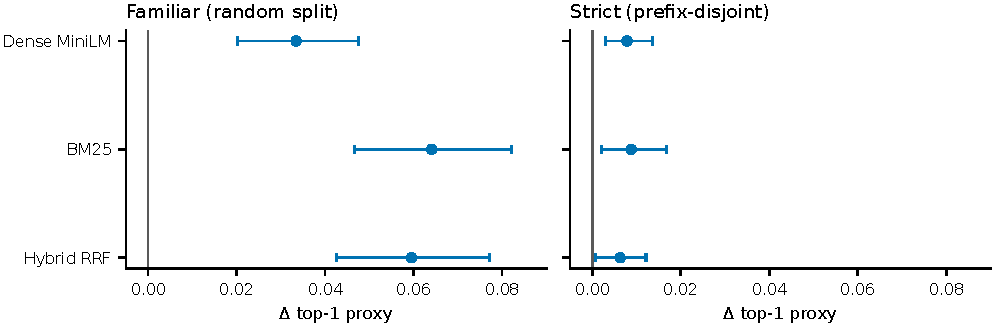
\includegraphics[width=\textwidth]{revision_ieee_access/03_manuscript/figures/fig5_matched_retrievers.pdf}
\caption{Feedback gain under one configuration (EB $\kappa=2$, pool-relative
scaling $\lambda=1$) for dense MiniLM, BM25 and hybrid RRF. Bars are 95\,\%
bootstrap intervals. The earlier claim that stronger retrieval reduces the benefit
is not supported once the lift configuration is held fixed.}
\label{fig:matched}
\end{figure*}

The feedback gain is similar across retrieval families: on the familiar panel
$+0.0334$, $+0.0641$ and $+0.0595$; on the strict panel $+0.0078$, $+0.0088$ and
$+0.0063$. The earlier conclusion that stronger retrieval reduces the benefit is a
scaling artefact: absolute lift units are cosine units and are not meaningful on
BM25 scores. We withdraw that conclusion. This article does not claim that
retriever choice is irrelevant; it claims that the earlier comparison could not
separate retriever strength from lift scale.

\subsection{Mechanism}
The blind failure is arithmetic before it is statistical. The judge is
negative-heavy: on the allowed strict rows, 62.9\,\% of conditioned and 57.3\,\% of
blind scores are negative, against 12.1\,\% and 7.8\,\% positive. With zero
positive and two negative votes, Eq.~\ref{eq:legacy} gives $p=0.25$ and
$\ell=(0.25-0.5)\cdot1\cdot0.8=-0.20$, exactly the negative cap. More negatives
change nothing: two negative votes and twenty receive the same penalty. The
formula is antisymmetric, and two positive votes with no negatives reach the
positive cap in exactly the same way. The observed asymmetry is therefore a
property of the evidence distribution, not of the prior: the judge supplies many
more negatives than positives.

Figure~\ref{fig:saturation} measures the consequence. Under the legacy lift,
13.2\,\% of conditioned candidates with two votes sit at the negative cap and
0.15\,\% at the positive cap; for blind, the shares are 9.1\,\% and 0\,\%. At five
votes the negative-cap share is 15.6\,\% (conditioned) and 7.0\,\% (blind), while
the positive-cap share is 0\,\%. The cap turns the bonus into a near-constant
penalty for a large part of the pool. In the strict dev ablation, the
empirical-Bayes negative-cap share is 7.9\,\% and the positive cap remains
negligible.

\begin{figure*}[!t]
\centering
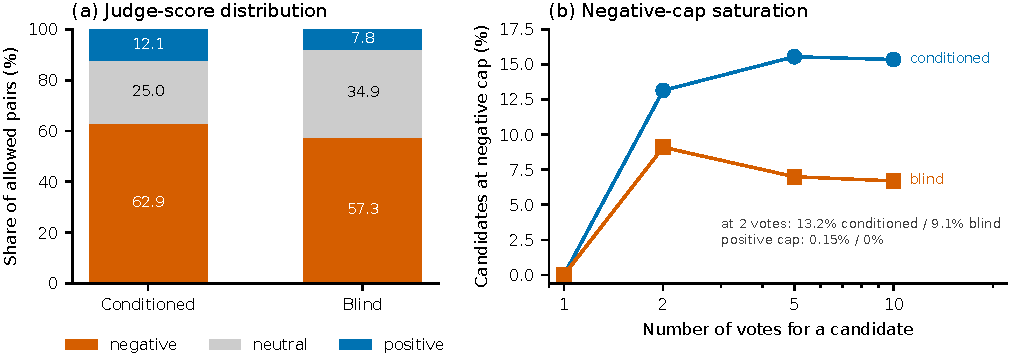
\includegraphics[width=\textwidth]{revision_ieee_access/03_manuscript/figures/fig4_lift_saturation.pdf}
\caption{Lift saturation. (a)~Judge-score distribution on the allowed strict rows:
negative, neutral and positive shares for conditioned and blind feedback. (b)~Share
of candidates at the negative cap as a function of the number of votes. The
negative-cap mass is a property of the evidence distribution interacting with the
legacy ramp; the positive cap is negligible in both protocols.}
\label{fig:saturation}
\end{figure*}

\subsection{Control as risk control}
The gate is not a source of gain. It pays when the uncalibrated prior concentrates
harm and becomes mostly redundant once the prior is repaired. On the strict blind
panel, always-on is $+0.0008$ and the hindsight upper bound is $+0.0190$, so the
maximum headroom is 0.0182. On the familiar blind panel, always-on is $-0.0444$ and
the hindsight bound is $+0.0258$, headroom 0.0701. A feasible gate can capture only a
fraction of that headroom, and we do not claim that it recovers the ceiling. In the
earlier evaluation, the gate was trained once across signals and protocols with
grouped cross-validation by ticket; its dev out-of-fold AUC was 0.699
$[0.676,0.721]$, and eval AUC ranged from 0.56 to 0.74. The feature-family
ablation showed that intervention shape carried the signal (AUC 0.681), while
baseline quality (0.553), semantic cosine (0.548) and scope evidence (0.548) added
little. This is consistent with the mechanism: the gate
predicts pool reshaping, not similarity.

The expected-value analysis in the earlier evaluation pooled conditioned and blind
rows, which are two per ticket and not independent. We do not use that analysis for
a main claim. It is reported in the Appendix as exploratory, with the
non-independence caveat, and it is not used to compare a protocol a deployed system
cannot run with one it can.
